\authoredSection{marco}{Ergebnis}
\vspace{-24pt}
\begin{figure}[h!]
	\centering
  	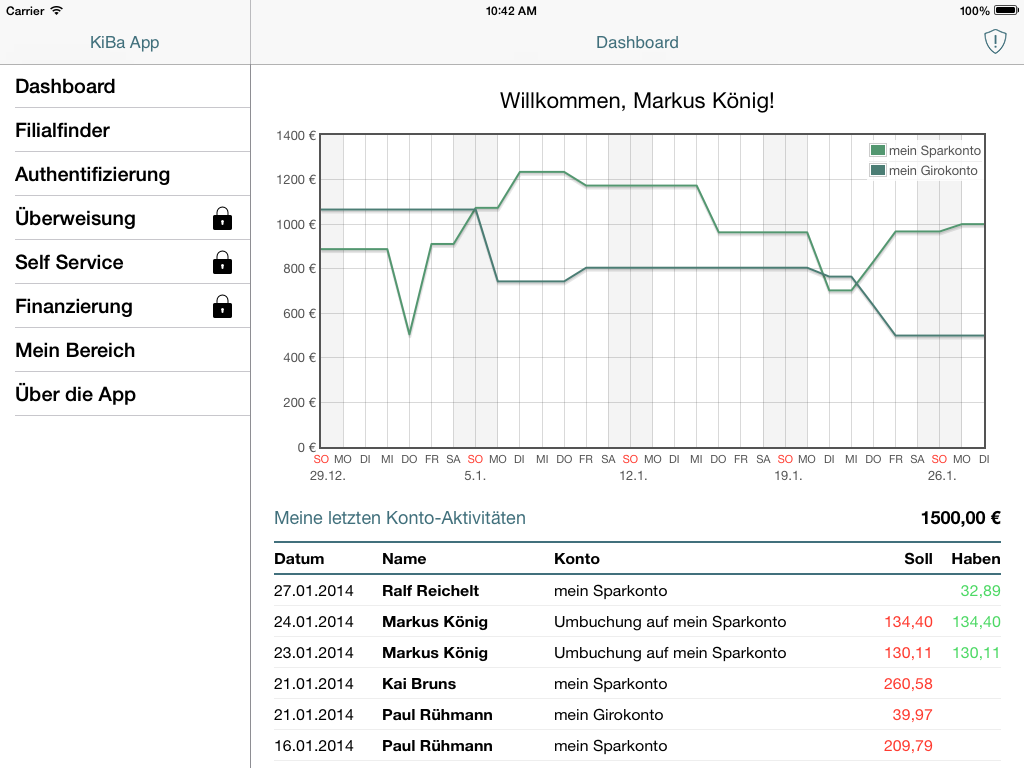
\includegraphics[height=0.25\textheight]{Pictures/Dashboard}
	\vspace{-12pt}	
	\caption{Screenshot des Dashboards}
	\label{fig1}
\end{figure}
\vspace{-12pt}
\begin{figure}[h!]
	\centering
	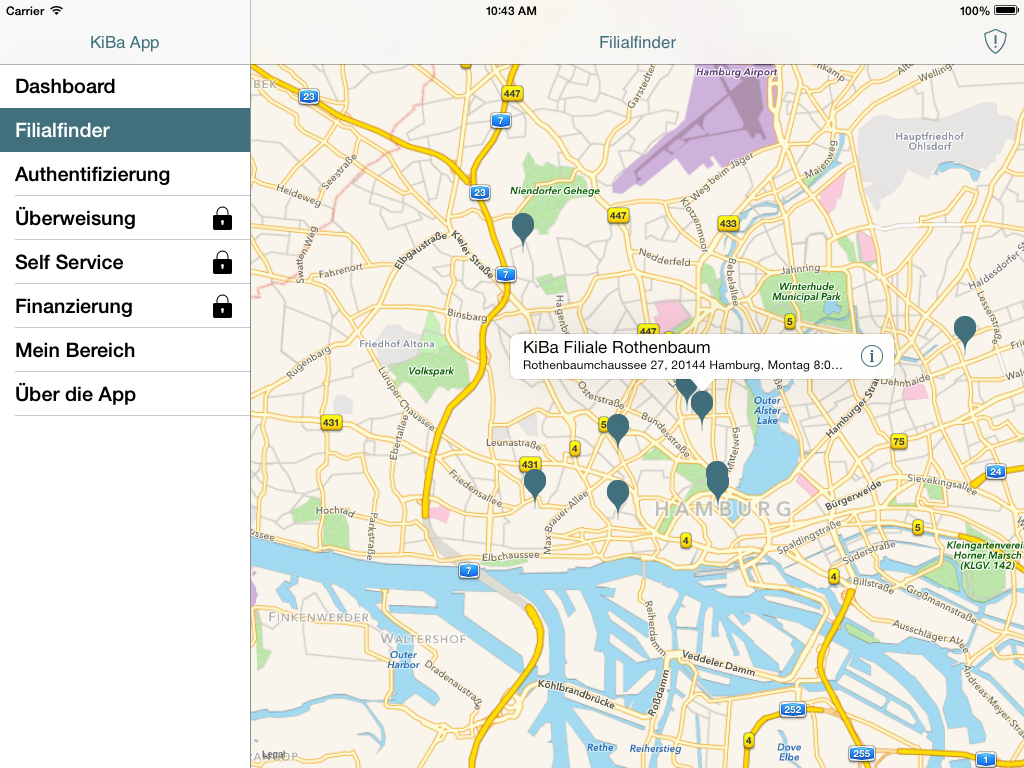
\includegraphics[height=0.25\textheight]{Pictures/filialfinder}
	\vspace{-12pt}	
	\caption{Screenshot des Filialfinders}
	\label{fig2}
\end{figure}
\vspace{-12pt}
\begin{figure}[h!]
	\centering
	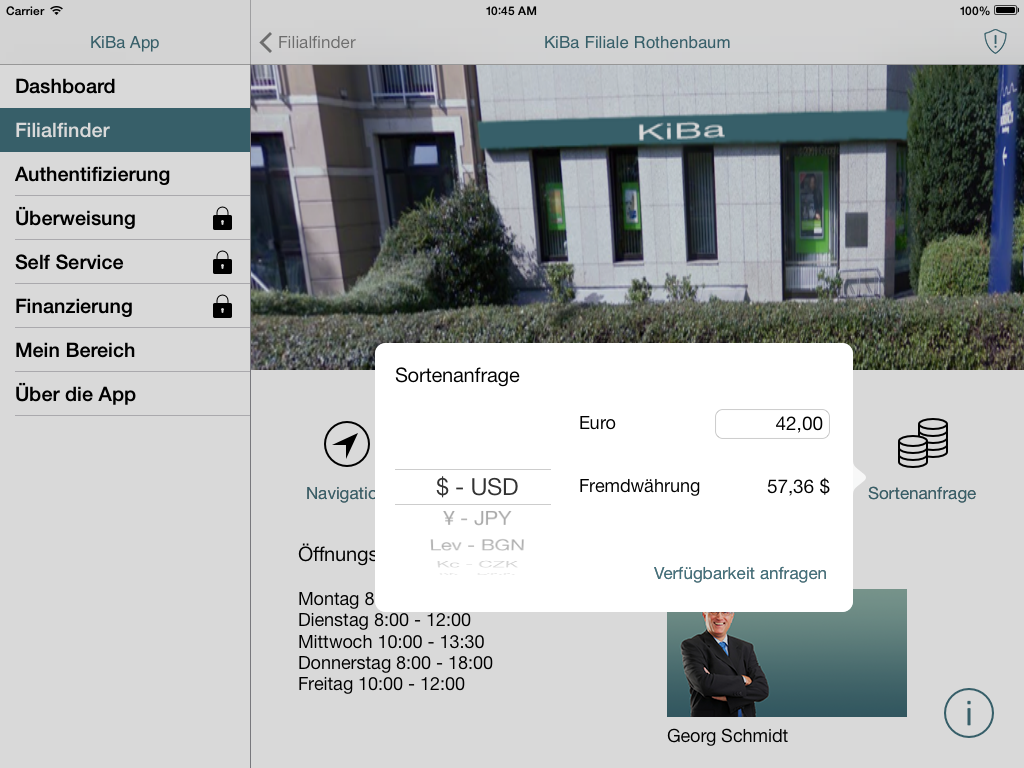
\includegraphics[height=0.25\textheight]{Pictures/Sortenanfrage}
	\vspace{-12pt}
	\caption{Screenshot der Filialseite mit Sortenanfrage Pop-Over}
	\label{fig3}
\end{figure}

\pagebreak
\subsection{Features}
\subsubsection{Dashboard}
Das Dashboard ist die zentrale Anlaufstelle der Applikation; dort haben wir einen Überblick über den Verlauf der Kontostände aller unserer Konten. In der Tabelle darunter haben wir die Möglichkeit, alle Kontobewegungen nachzuverfolgen.

\subsubsection{Filialfinder}
	Beim Filialfinder findet man eine Karte von Apple Maps mit Markierungen, welche die Standorte der einzelnen Filialen markieren. Mit einem Klick auf das Infosymbol gelangt man zu einer Filialseite, auf der man die Öffnungszeiten nachschauen, aber auch eine Terminanfrage oder eine Sortenanfrage stellen kann.

\subsubsection{Sortenanfrage}
	Mit einem Klick auf Sortenanfrage bekommt der Nutzer ein Pop-Over zu sehen, in welchem er seine Wunschwährung auswählen kann. Die entsprechenden Umrechnungskurse werden intern direkt von der Europäischen Zentralbank bezogen. Hat man die Summe, welche umgetauscht werden soll eingegeben, so kann man die Anfrage stellen und bekommt eine Nachricht, ob die gewünschte Währung in der gewünschten Höhe bei der gewünschten Filiale verfügbar ist.

\subsubsection{Authentifizierung}
\begin{figure}[h]
    \centering
	\begin{tabular}{@{}cc@{}}
        	
\includegraphics[width=1.5cm]{Pictures/notauth} &
    		
\includegraphics[width=1.5cm]{Pictures/authed}
    \end{tabular}
	\caption{Die Authentifizierungsstati\label{fig4}}
\end{figure}
\pagebreak
\noindent	Im oberen rechten Rand der Applikation ist ein kleines Symbol in Form eines Schildes zu sehen; dieses gibt den Authentifizierungsstatus zurück. Ein Schild mit einem Ausrufezeichen symbolisiert eine fehlende Authentifizierung, ein Haken eine gültige Authentifizierung.

	Solange das Gerät nicht authentifiziert ist, kann man einige Funktionen nicht benutzen, diese sind durch das Symbol mit dem geschlossenen Schloss gekennzeichnet.

	Unter dem Menüpunkt Authentifizierung findet man ein kleines Comic vor. Dieses erläutert, wie der Nutzer sein Gerät bei seiner Filiale authentifizieren kann. Außerdem wird der Nutzer auf seine Vorteile aufmerksam gemacht.

\subsubsection{Überweisung}
	Unter dem Menüpunkt Überweisung findet man ein ganz gewöhnliches Überweisungsformular, die Überweisung muss man abschließend noch mit einer TAN bestätigen.

\subsubsection{Self-Service-Station}
\begin{figure}[h]
	\centering
  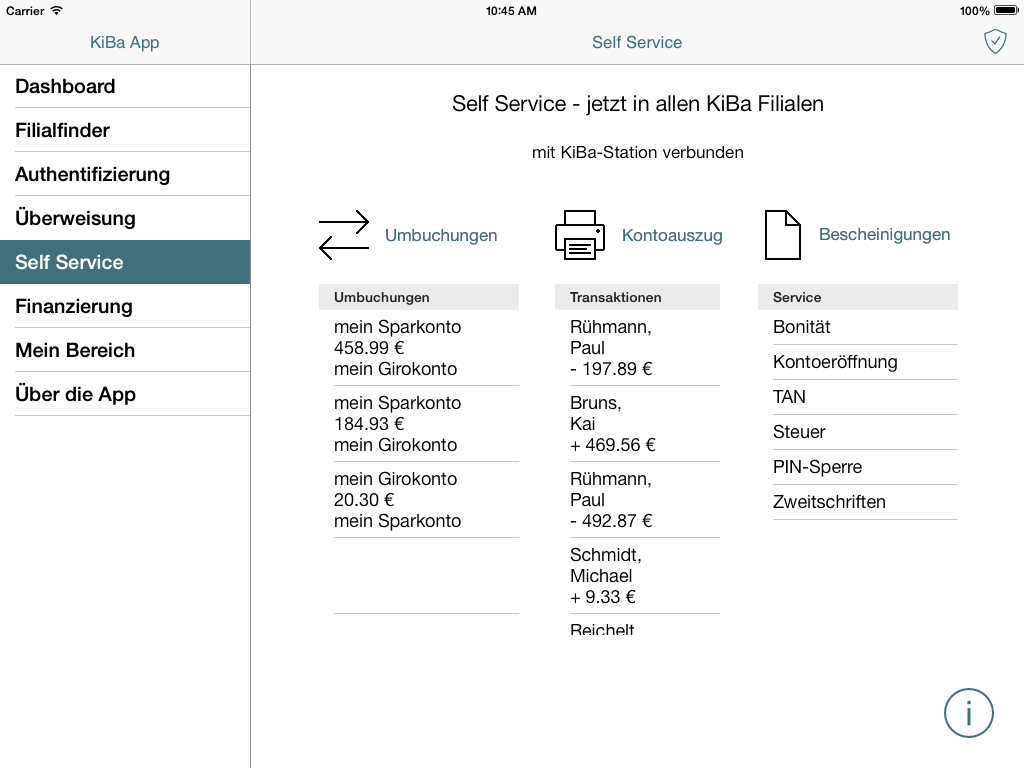
\includegraphics[width=0.5\textwidth]{Pictures/SSverbunden}
	\caption{Self-Service Startseite. Die App ist verbunden.}
	\label{fig5}
\end{figure}

\noindent	Bei der Self-Service-Station haben wir die Möglichkeit, sofern wir mit dem Stationsgerät verbunden sind, drei verschiedene Aktionen eigenständig durchzuführen. Eine Umbuchung, Kontoauszüge anschauen und drucken, sowie Bescheinigungen ansehen, ausfüllen und ausdrucken gegeben falls direkt abschicken.

	Jede Auswahlmöglichkeit hat eine Tabelle mit Inhalten, die den User erwarten, wenn er auf den entsprechenden Button drückt.

\subsubsection{Bescheinigungen}
\begin{figure}[h]
	\centering
  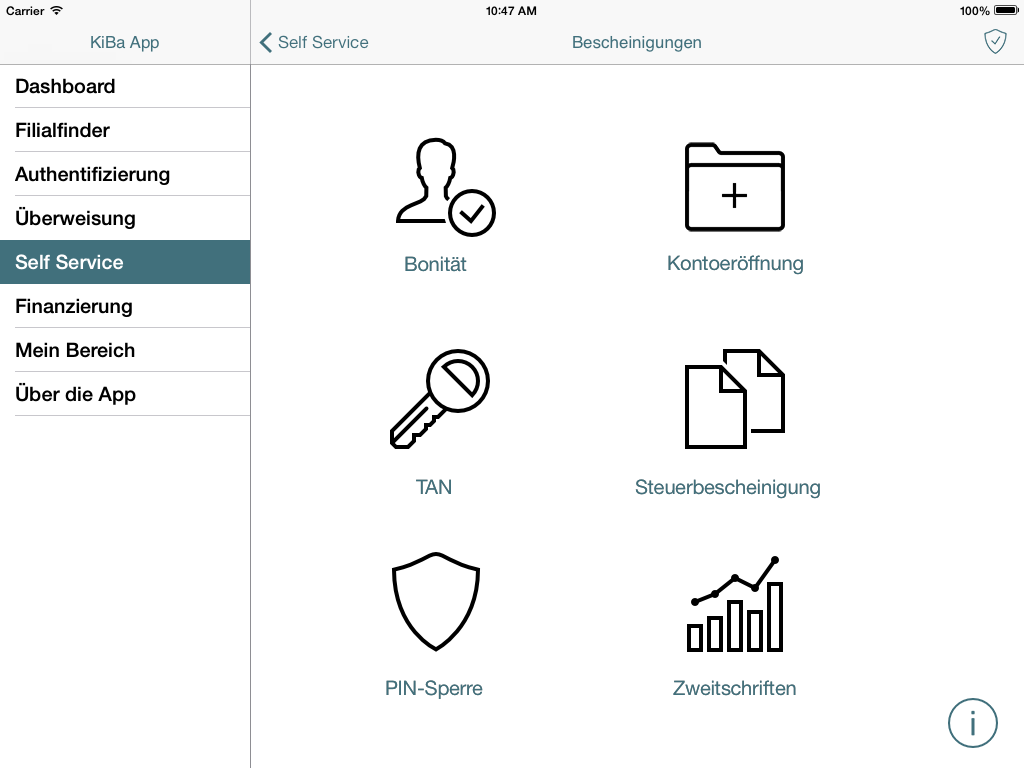
\includegraphics[width=0.5\textwidth]{Pictures/Bescheinigungen}
	\caption{Die verschiedenen Dokumenttypen}
	\label{fig6}
\end{figure}

	Bei den Bescheinigungen sehen wir verschiedene von der Bank zur Verfügung gestellte Dokumente, die der Nutzer auswählen kann. Insbesondere beispielsweise sind Aktionen wie eine Kontoeröffnung möglich, für die man normalerweise am Schalter anstehen müsste.

\subsubsection{Kontoauszüge}
\begin{figure}[h]
	\centering
  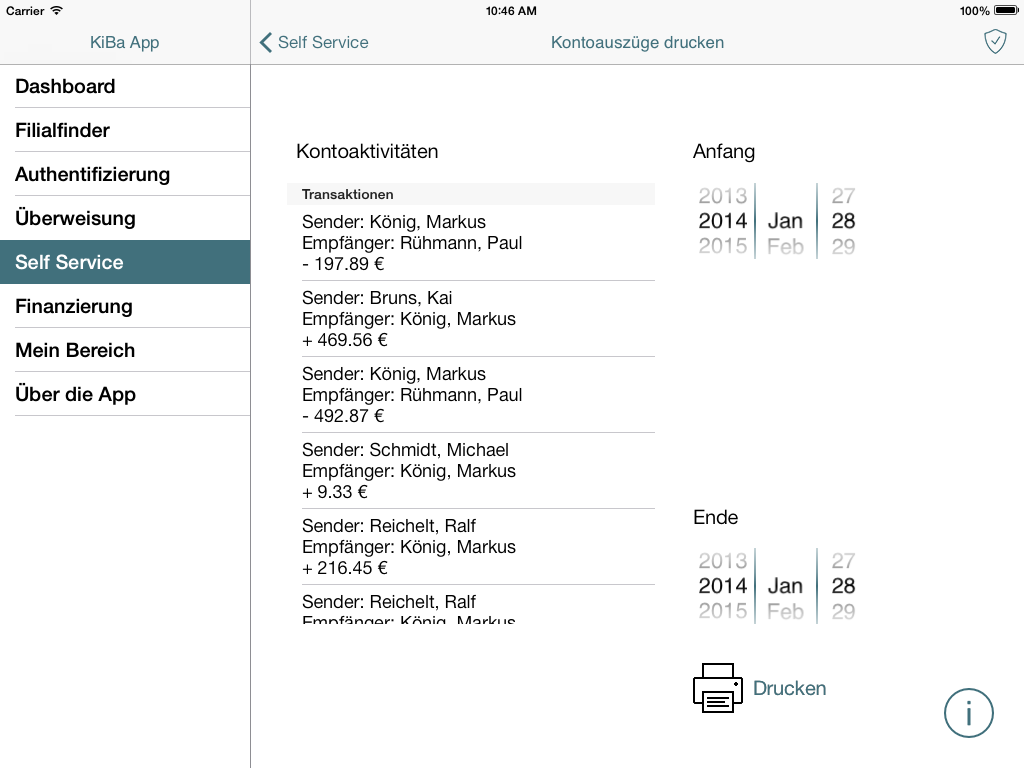
\includegraphics[width=0.5\textwidth]{Pictures/kontoauszuege}
	\caption{Übersicht der Kontoauszüge}
	\label{fig7}
\end{figure}

	Im Kontoauszugsbildschirm kann man Kontoaktivitäten in einem bestimmten Zeitraum drucken lassen. Somit integriert die Station den althergebrachten Kontoauszugsdrucker und gibt ihm eine zeitgemäßere Oberfläche.

\subsubsection{Umbuchungen}
\begin{figure}[h]
	\centering
  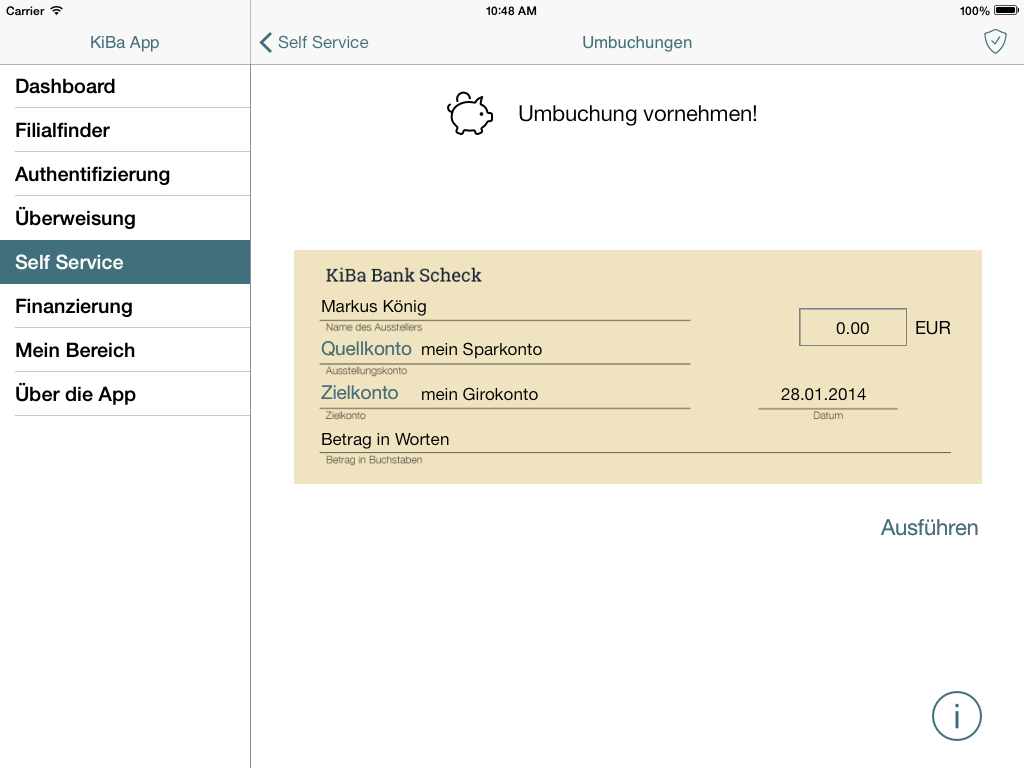
\includegraphics[width=0.5\textwidth]{Pictures/umbuchung}
	\caption{Eine Scheckgrafik als Formular für die Umbuchung}
	\label{fig8}
\end{figure}

	Im Umbuchungsbildschirm kann der Nutzer sowohl Ziel- als auch Quellkonto auswählen, zwischen denen der angegebene Betrag transferiert werden soll. Das Ganze wird mit einem Button bestätigt. Insbesondere wird hier das klassische Sparbuch um eine komfortable Umbuchungsfunktionalität erweitert, ohne dass dessen filialgebundener Charakter verloren ginge.

\subsubsection{Finanzierungsrechner}
\begin{figure}[h]
	\centering
  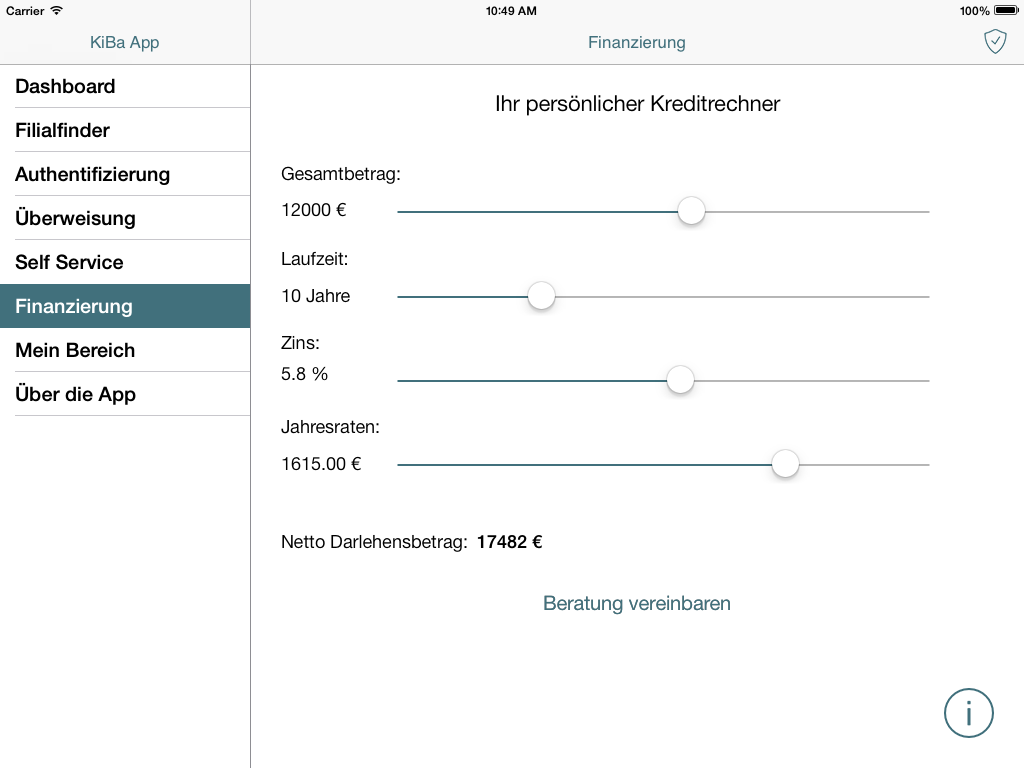
\includegraphics[width=0.5\textwidth]{Pictures/finanzierung}
	\caption{Finanzierungsrechner mit individuellen Konditionen}
	\label{fig9}
\end{figure}

	Mit dem Finanzierungsrechner kann man sich Kreditkonditionen zusammenstellen. Die Werte der einzelnen Schieberegler werden aus dem Profil des Kundens von der Bank vorgegeben.

	Man kann danach auch wieder einen Beratungstermin vereinbaren um die Konditionen mit seinem Berater nochmal durchsprechen zu können, inwiefern die ausgewählten Konditionen empfehlenswert für den Kunden sind oder ob die Bank vielleicht noch bessere Sonderkonditionen anbieten kann.

\subsubsection{Mein Bereich}
%Nachrichtensystem
%mbereichneu.png

\begin{figure}
	\centering
  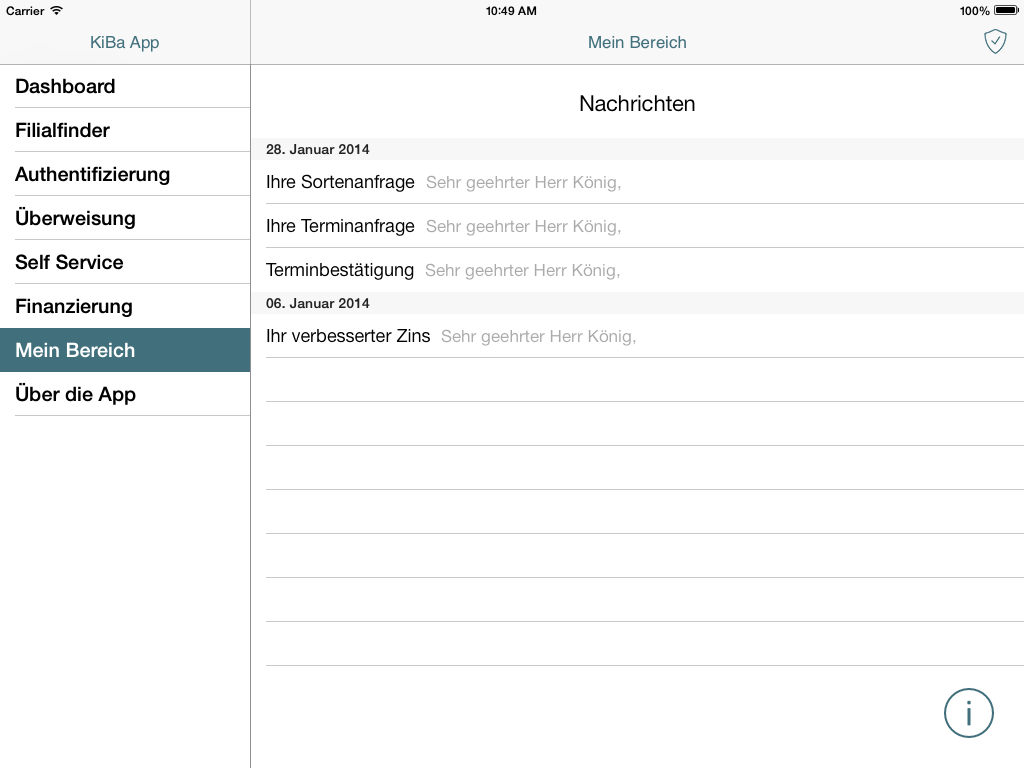
\includegraphics[width=0.5\textwidth]{Pictures/mbereichneu}
	\caption{Ein minimalistischer Posteingang des Nutzers\label{fig10}}
\end{figure}

	Der Nutzer kann in seinem persönlichen Bereich Nachrichten der Bank empfangen und somit beispielsweise eine Bestätigung für seine Terminanfrage erhalten. Mit einem Klick auf die Zelle einer Nachricht bekommt man die entsprechende Nachricht in einer neuen Ansicht mit dem kompletten Nachrichtentext.

\subsection{Die Design-Highlights}
\begin{figure}[h!]
	\centering
    \begin{tabular}{@{}ccc@{}}
    		\framebox{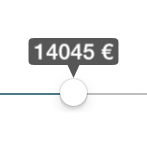
\includegraphics[width=2.5cm]{Pictures/DesignA}} &
    		\framebox{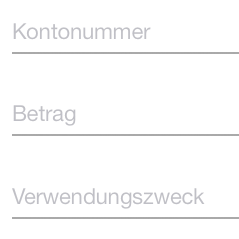
\includegraphics[width=2.5cm]{Pictures/DesignC}} &
    		\framebox{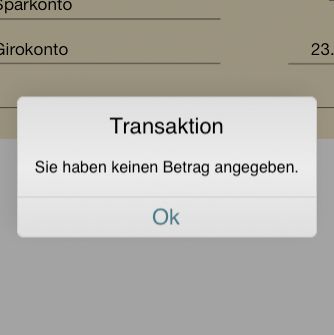
\includegraphics[width=2.5cm]{Pictures/DesignB}} \\
    		A & B & C
    \end{tabular}
	\caption{Eigenkreationen für das Design\label{fig11}}
\end{figure}

Um unsere Applikation in mancher Hinsicht besser auf unsere Bedürfnisse anzupassen, haben wir bei einigen Designelementen die Standardimplementierungen von Apple ergänzt. Dennoch blieben die iOS 7 Richtlinien ein Qualitätsmaßstab für uns.

Wie in (A) zu sehen ist, bekam unser Schieberegler als kleine Erweiterung eine schwarze Sprechblase, welche den aktuellen Wert anzeigt. Dies ist im Speziellen unter dem Gesichtspunkt der Bedienbarkeit implementiert worden, damit man beim Verschieben des Regler nicht immer auf die linke Seite schauen muss um den aktuellen Wert abzulesen.

Die mitgegebenen Textfelder von Apple haben in der Regel immer einen Text, welcher dem Nutzer einen Hinweis gibt, was für ein Inhalt erwartet wird. Diese Umsetzung sieht oftmals unschön aus und nimmt viel Platz ein. Mit unserer Implementierung (B) verliert das Textfeld keine Funktionalität, ist aber schlanker.

Die Standard Pop-Over lassen sich nur bedingt anpassen. So konnten wir die Farbe des Buttons nicht in unserem Farbton einfärben. Daher mussten wir auf eine Eigenimplementation (C) zurückgreifen um die Konsistenz zu wahren.

% Pop Over
% Sliderinfo
% mehr custom!!!!

\subsection{Herausforderungen}
	Mit zu den größten Herausforderungen war das Design der einzelnen Bildschirme. Das „Flat“-Design braucht ein gutes Händchen und kleine Details können schon zu Unstimmigkeiten führen. Gleichzeitig war uns bewusst, dass wir eine Bank repräsentieren und somit ein gewisses Maß an Seriosität erforderlich war. Gleichzeitig mussten wir die Usability für den Endnutzer gewährleisten. Wir mussten ein App-Design erschaffen, welches drei Stakeholder gleichzeitig zufriedenstellt.

%Die größte Herausforderung war aber ein sogenanntes „Killer“-Feature zu erschaffen. Nach unseren Erkenntnissen gibt es keine herausragende Eigenschaft der Filialbank, welche sie von Direktbanken unterscheidet. Vor allem nach der Finanzkrise ab 2007 ist das Vertrauen in Filialbanken stark gesunken, davor war die persönliche Beratung immer das Unterscheidungsmerkmal zu Direktbanken.
%Es bleibt nur noch die Finanzierung übrig, doch diese wird nur von einem Bruchteil der Kunden in Anspruch genommen. Berücksichtigt man noch die Anstrengungen der Direktbank auch eine persönliche Beratung per Telefonhotline anzubieten, indem der Kunde immer den gleichen Berater am Apparat hat, dann sieht man, dass selbst diese Lücke langsam aber sicher von den Direktbanken geschlossen wird.
%
%Wir als Entwickler konnten natürlich die Bank in ihrem Wesen nicht verändern, die Einführung von neuer Hardware mit der Self-Service Station war schon das Maximum an Veränderung die wir Einfordern konnten.

	Mit einer neu zu erlernenden Programmiersprache und deren Entwicklungsumgebung geht auch immer eine Herausforderung einher. Die ersten Wochen hatten wir somit erwartungsgemäß etwas geringere Produktivität, weil wir uns auf diese Gegebenheiten erst einstellen mussten. Je weiter jedoch das Projekt voranschritt, desto sicherer fühlten wir uns in Objective-C und im Umgang mit Xcode.

	Während der Entwicklung stießen wir auch immer wieder auf Einschränkungen seitens Apple bezüglich der Standard GUI-Elemente. So konnten wir beispielsweise die Tint-Color eines Buttons im Pop-Over nicht ändern. Apple lässt dies nicht zu. Daher mussten wir hier unser eigenes Pop-Over implementieren.

	Nichtsdestotrotz konnten wir mit Unterstützung der Betreuer alle größeren und kleineren Herausforderungen bewältigen und hatten nie das Gefühl, vor einem unüberwindbaren Problem zu stehen.